\label{sec:Sentiment}

Eines der Ziele von TMetrics ist es, ein umfassendes und detailliertes Meinungsbild zu einem Thema zu erstellen. Diesem Zweck dient die Sentimentanalyse: die „rechnerische Handhabe von Meinungen, Sentiment und Subjektivität in Text"' \cite{Pang2008}. Unter Sentiment wird dabei ein Gefühl verstanden, das sich auf ein bestimmtes Ziel richtet, beispielsweise Ablehnung oder Zustimmung zu einer politischen Meinung.

Die Datenmengen, die in modernen sozialen Medien anfallen und die auch als "`Big Data"' verschlagwortet worden sind, machen eine manuelle Analyse impraktikabel. Sentimentanalyse auf Twitterkommunikation anzuwenden heißt also, die themenspezifischen Meinungen einer Gruppe von Menschen automatisiert zu analysieren und zu quantifizieren. Dabei wird die Annahme zugrundegelegt, dass sich der emotionale Gehalt eines Tweets in einer trinären Klassenzuordnung (gut, neutral, negativ) oder einer Zahl von -1 bis +1, im Folgenden Sentimentwert genannt, ausdrücken lässt.

Im Unterabschnitt \ref{subsec:sentimenttheorie} werden eine Reihe von theoretischen Modellen vorgestellt, um den Sentimentwert eines Texts zu bestimmen. Im Unterabschnitt \ref{subsec:sentimentimplementierung} wird das Java-Paket beschrieben, in dem diese Modelle implementiert wurden. Im Unterabschnitt \ref{subsec:sentimentimplementierung} wird schließlich beschrieben, wie die Berechnung der Sentimentwerte in diesem Paket in die restliche Architektur mit Daemon und REST-Service eingebunden ist und wie die Sentimentwerte schließlich im Front-End angezeigt werden.

\subsection{Theoretische Grundlagen}
\label{subsec:sentimenttheorie}

Eine simple Methode, den Sentimentgehalt eines Tweets näherungsweise zu bestimmen, wird von Twitter selbst verwendet. Es werden eine Liste von positiven Emoticons und eine Liste von negativen Emoticons erstellt. Wenn ein positives Emoticon im Tweet enthalten ist, wird der Tweet als positiv aufgefasst; ist ein negatives Emoticon enthalten, wird er als negativ verstanden. Im Beispielsatz "`I love puppies :-)"' wird beispielsweise das "`:-)"' als positiv erkannt. Diese Methode ist einfach und nach unserer Erfahrung in der Hinsicht einigermaßen verlässlich, dass tatsächlich die meisten so identifizierten Tweets positiv sind. Allerdings ist sie ungeeignet, um ein detailliertes Meinungsbild zu erstellen, weil nur ein Bruchteil aller Tweets überhaupt ein Emoticon enthält.

Statt Listen von positiven und negativen Emoticons lassen sich Listen von Wörtern verwenden. Wörterbücher dieser Art sind aufwändig zu erstellen, da sie oftmals tausende von Wörtern enthalten, aber einige solcher Listen sind frei im Internet verfügbar. Im Satz "`I love puppies :-)"' wird mithilfe eines Wörterbuchs beispielsweise das "`love"' als positiv erkannt. Die Bewertungen der Einzelwörter werden dann aggregiert, um eine Bewertung des Textes zu berechnen.

Ein naiver Wörterbuchansatz allein ist allerdings ebenfalls ungeeignet, den Sentimentwert eines Tweets zu bestimmen. Zum Beispiel würde ein Wörterbuch in der Kombination "`not good"' ein positives Wort sehen. Auch Redewendungen und Ironie werden so nicht erkannt. Daher werden teils zusätzlich Listen von Phrasen verwendet, oder die Wörterbücher werden gemeinsam mit Regelwerken verwendet, um z.\,B. den Sentimentwert eines Wortes umzukehren, das auf "`not"' folgt. Auch solche Regelwerke müssen von Menschen mühevoll erstellt werden. Angesichts der Komplexität natürlicher Sprachen verwundert nicht, dass sie fehleranfällig und unvollständig sind.

Eine Forschungsdisziplin, die Abhilfe verspricht, ist die des maschinellen Lernens (\textit{machine learning}). Im Gegensatz zu Emoticon- und Wörterbuch-Listen und Regelwerken müssen Zusammenhänge hier nicht mehr von Menschen explizit formuliert werden, um dann von der Maschine für deduktive Schlussfolgerungen verwendet zu werden. Stattdessen lernt die Maschine induktiv anhand von Beispielen. Das so gewonnene "`Wissen"' erlaubt nach der Trainingsphase die Klassifikation neuer Daten anhand von Beispielen. Die Erstellung dieser Beispiele, Trainingsdaten genannt, ist wesentlich leichter als die Erstellung komplexer Regelwerke. Tabelle \ref{sentiment:trainingdata} zeigt zwei Beispielsätze, die als Trainingsdaten dienen können.

\begin{table}
 \centering
\caption{Trainingsdaten}\label{sentiment:trainingdata}
\begin{tabular}{lc}
Text & Sentiment \\
I love puppies & \textcolor{green}{\(+1\)} \\
I hate puppies & \textcolor{red}{\(-1\)} \\
\end{tabular}
\end{table}

Im Gebiet des maschinellen Lernens werden eine Reihe von Algorithmen angewandt. Dazu zählen zum Beispiel lineare und logistische Regression, \textit{Support Vector Machines} und neuronale Netzwerke. Im Rahmen dieses Projekts fiel die Entscheidung auf die Implementierung der linearen Regression. Die Wahl eines vergleichsweise einfachen Algorithmus erlaubte es uns, diesen vollständig und korrekt selbst zu implementieren, anstatt auf eine vorhandene Implementierung in Form einer Bibliothek zurückgreifen zu müssen. Dies war im akademischen Kontext mit der Zielsetzung eines möglichst großen Lerneffekts erwünscht.

Der linearen Regression liegt folgendes Modell zugrunde:
\[ y = h_{\theta} (x) + \epsilon = \theta_0 x_0 + \theta_1 x_1 + \cdots + \theta_n x_n + \epsilon \]
Für jeden Trainingsdatensatz ist \( y \) das tatsächliche Sentiment des Texts, das anhand der Merkmale \( x_1 \cdots x_n \) vorhergesagt werden soll (\( x_0 = 1 \)). Die Werte der Parameter \( \theta_0, \cdots, \theta_n \) sind unbekannt. Der Fehlerterm \( \epsilon \) gibt die Abweichung der Schätzung anhand der Merkmale und Parameter vom tatsächlichen Wert an. Betrachtet man alle Trainingsdaten gleichzeitig, kommt die vektorisierte Form der Gleichung zum Einsatz:
\[ y = h_{\theta} (x) + \epsilon = X \cdot \theta + \epsilon \]
y und \( \epsilon \) sind jetzt Vektoren. X ist eine Matrix, die Merkmals- oder Featurematrix, die in den \( m \) Zeilen die einzelnen Trainingsdaten enthält. Die \( n + 1 \) Spalten sind die einzelnen Merkmale. Die Einträge der Matrix geben an, ob und in welcher Quantität ein Merkmal in einem Trainingsdatensatz vorliegt. Tabelle \ref{sentiment:matrix} zeigt die Merkmalsmatrix.

\begin{table}
 \centering
\caption{Trainingsdaten als Merkmalsmatrix}\label{sentiment:matrix}
\begin{tabular}{cccc|c}
I & love & hate & puppies & Sentiment \\
1 & 1 & 0 & 1 & \textcolor{green}{\(+1\)} \\
1 & 0 & 1 & 1 & \textcolor{red}{\(-1\)} \\
\end{tabular}

\end{table}

Die Aufgabe der linearen Regression besteht nun darin, die Einträge im Fehlervektor \( \epsilon \) zu minimieren. Dies geschieht typischerweise mit der Methode der kleinsten Quadrate, d.\,h. die Summe der Quadrate der Fehlerterme soll minimal werden:
\[ \min \frac{1}{2m} \sum_{i=1}^{m} (h_{\theta} (x^{(i)}) - y^{(i)})^2 \]

Für die Suche nach dem Minimum dieser Funktion existiert eine geschlossene Lösung, die jedoch eine Matrixinversion einer $n\times n$-Matrix erfordert mit $n$ als Anzahl der Merkmale. Da Matrixinversionen typischerweise eine Laufzeit in \( \mathcal O(n^3) \) hat und $n$ schon bei der Verwendung von Unigrammen (Wörtern) als Merkmalen schon bei einigen hundert Tweets eine Zahl im Tausenderbereich erreicht, ist dieser Algorithmus für die Sentimentanalyse ungeeignet.

Eine Alternative ist das Gradientenabstiegsverfahren, bei dem zu Beginn beliebige Parameterwerte gewählt werden (z.\,B. $0$ für jeden Parameter) und das in jeder Iteration einen kleinen Schritt in Richtung des Gradienten macht, d.\,h. die Parameterwerte bei jeder Iteration so verändert, dass der Funktionswert geringer wird. Diese Methode läuft zwar Gefahr, zu einem lokalen Optimum zu  konvergieren, ohne das globale Optimum zu finden. Da aber die Kostenfunktion konvex ist, d.\,h. keine lokalen Minima außer dem globalen Minimum hat, kann man diese Schwäche hier vernachlässigen. Im Gradientenabstiegsverfahren werden in jeder Iteration \( i \) die Sentimentwerte mit den aktuellen Parameterwerten geschätzt und die neuen Parameterwerte wie folgt berechnet:

\begin{algorithm}
 \caption{Gradientenabstiegsverfahren für die lineare Regression}\label{sentiment:gradientdescent}
\begin{algorithmic}[1]
\Statex \textbf{Eingabe:} $ \mathbf{X}\in \mathbf{R}^{m \times n + 1} $ Merkmalsmatrix mit den Einträgen $ x_{j}^{i} $, $ \epsilon $ Konvergenzmaß, $ \alpha $ Schrittweite
\Statex \textbf{Ausgabe:} $\mathbf{\theta}\in \mathbf{R}^{n + 1}$ Parametervektor mit den Einträgen \( \theta_{j} \)
\For{$(j = 1; j < n + 1; j++)$}
\State $ \theta_j = 0 $
\EndFor
\State $ e_{current} = \inf $
\Repeat
\State $ h_{\theta} = X \cdot \theta $
\State $ e_{last} = e_{current} $
\State $ e_{current} = \frac{1}{2m} \sum_{i=1}^{m} (h_{\theta} (x^{(i)}) - y^{(i)})^2 $
\For{$(j = 1; j < n + 1; j++)$}
\State $ \theta_j = \theta_j - \alpha \frac{1}{m} \sum_{i = 1}^{m} (h_{\theta} (x^{(i)}) - y^{(i)})x_j^{(i)} $
\EndFor
\Until {$ e_{last} - e_{current} \leq \epsilon $}
\end{algorithmic}
\end{algorithm}

\subsection{Implementierte Klassifikatoren}
\label{subsec:sentimentimplementierung}

Abbildung \ref{sentimentuml} zeigt die Architektur des Java-Pakets \texttt{daemon.sentiment}. Es wurden nur die relevanten öffentlichen Methoden gekennzeichnet, um die Grafik übersichtlich zu halten.

\begin{figure}
 \centering


  \centering
    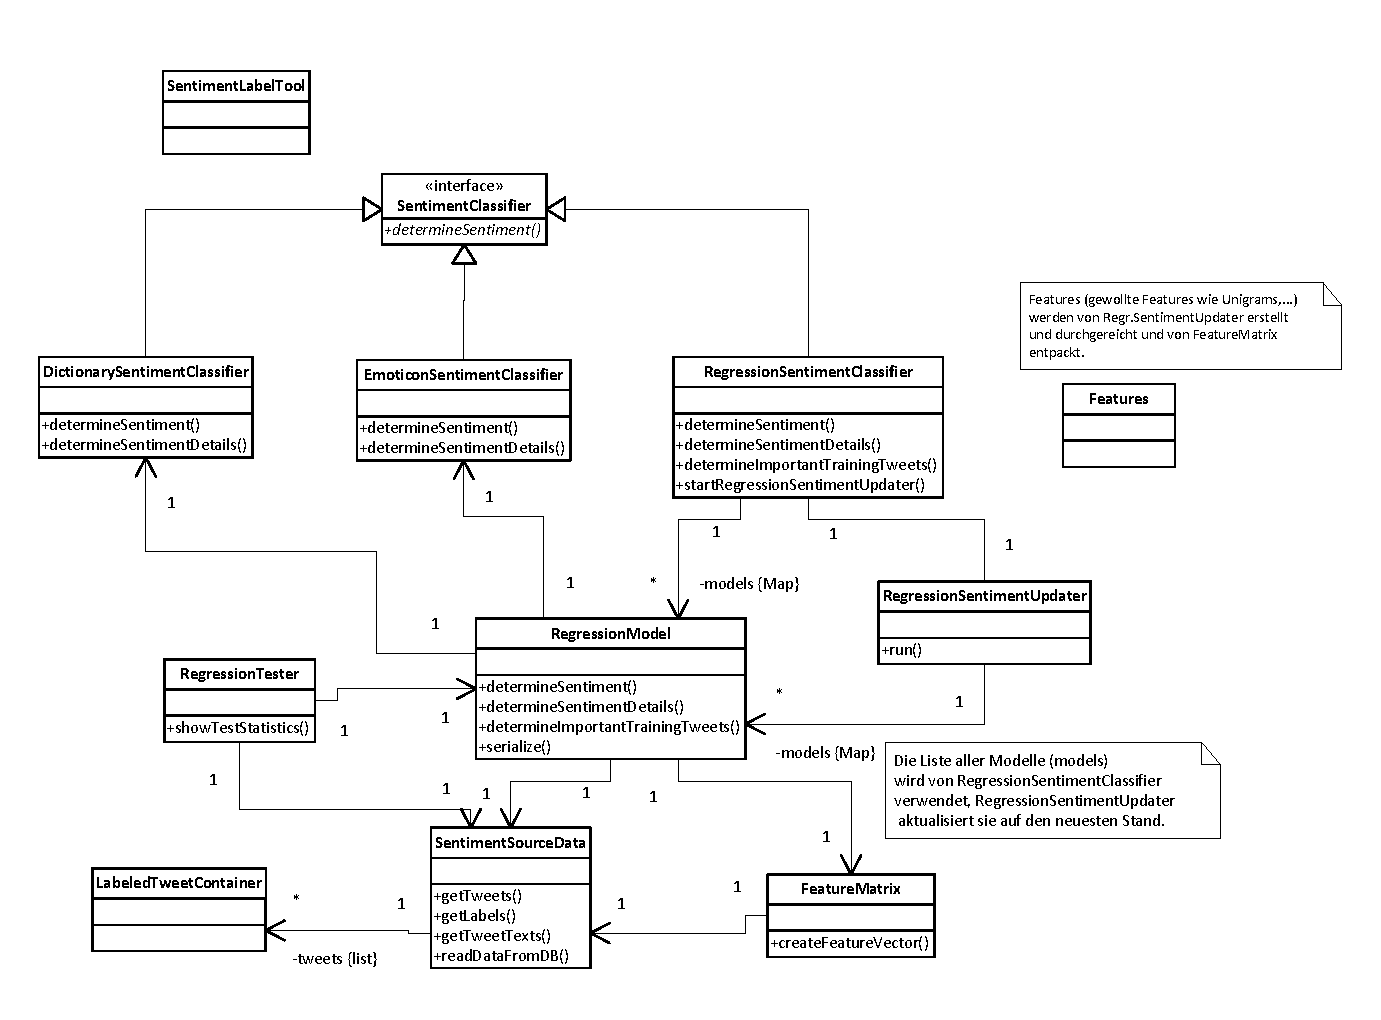
\includegraphics[width=\textwidth]{./Bilder/Sentiment/SentimentPackageClassDiagramm.pdf}
  \caption{Architektur des Pakets daemon.sentiment}
  \label{sentimentuml}
\end{figure}

Das Interface \texttt{Sentiment\-Classifier} definiert die Methode \texttt{determine\-Sentiment()}. Diese berechnet zu einem gegebenen Text in einer gegebenen Sprache den Sentimentwert. Drei Klassifikatoren implementieren dieses Interface, wobei jede der Implementierungen eine der vorgestellten Methoden umsetzt, Sentiment zu berechnen. Diese Klassen bilden die Schnittstelle des Sentiment-Pakets nach außen: Sie können von Daemon oder REST-Service instanziert werden (im Endprodukt wird der akkurateste Classifier, der \texttt{Regression\-Sentiment\-Classifier}, instanziert). Der Wörterbuch- und der Emoticon-Klassifikator erledigen alle anfallenden Aufgaben selbst. Der wichtigste Klassifikator, \texttt{Re\-gre\-ssion\-Sentiment\-Classifier}, greift zur Bewältigung seiner Aufgaben auf eine Reihe weiterer Klassen zurück, in deren Zentrum die Klasse \texttt{Regression\-Model} steht.

\subsubsection{Die Schnittstelle nach außen: Implementierungen von SentimentClassifier}
\label{sec:sentimentclassifier}

Der \texttt{Emoticon\-Sentiment\-Classifier} berechnet den Sentimentwert eines Textes auf Grundlage einer Emoticon-Liste, die in einem Abgleich mit dem Ergebnis der Twitter-Suche entstanden ist. Mit einer Twitter-Suche nach \textit{Merkel :-)} werden Tweets ausgegeben, die Twitter als positiv erkennt und die beispielsweise auch die Emoticons \textit{:-D} oder \textit{:-P} enthalten; analoges gilt für negative Tweets.

Der \texttt{Dictionary\-Sentiment\-Classifier} verwendet ein Wörterbuch, um den Sentimentwert eines Texts zu berechnen. Dabei kommen das ​Wörterbuch von Liu \cite{LiuLexicon}
 und die folgende Aggregierungsfunktion:

\[ \frac{\#pos - \#neg}{\#pos + \#neg} \]

Das Vorgehen ist damit dasselbe wie bei ​Stieglitz und Dang-Xuan (2012) \cite{Stieglitz2012}, allerdings mit einem anderen Wörterbuch, da das Wörterbuch von Liu im Gegensatz zum Wörterbuch des dort verwendeten Tools LIWC frei verfügbar ist. Beide beinhalten keine Gewichtungen für einzelne Wörter (z.\,B. ist "`super"' genauso positiv wie "`good"'), sodass die Aggregationsfunktion die Häufigkeit von positiven bzw. negativen Wörtern verwendet.

Das Wörterbuch wird "`roh"' verwendet, ohne grammatikalische Regeln, trotz der Warnung von Liu, dies nicht zu tun, sodass z.\,B. "`not happy"' positiv ist. Da aber vorgesehen ist, das Wörterbuch durch einen Machine-Learning-Algorithmus zu ersetzen, schien eine dahingehende Erweiterung der Wörterbuchklasse unsinnig.

Das Wörterbuch bewertet nur englischsprachige Tweets. Um zu erkennen, ob ein Tweet englischsprachig ist, wird der Rückgabewert der Twitter API-verwendet, die zu jedem Tweet einen zweistelligen ISO-Sprachcode liefert. Diese Klassifikation hat sich als ausreichend genau herausgestellt. Nicht-englischsprachige Tweets erhalten einen Sentimentwert von \texttt{null}. 

Die Klasse \texttt{Regression\-Sentiment\-Classifier} implementiert das Interface \texttt{Sentiment\-Classifier} und verwaltet die verschiedenen Regressionsmodelle. In einer Hashtabelle liegt für jede Sprache, für die genügend Trainings-Tweets vorliegen, ein Regressionsmodell. Als Schlüssel werden wiederum die zweistelligen ISO-Sprachcodes verwendet. Beim Start versucht der Classifier zunächst, bestehende, serialisierte Modelle von der Festplatte zu lesen und diese zu verwenden. Mit der Methode \texttt{start\-Regression\-Sentiment\-Updater()}, die vom Daemon aufgerufen wird, wird ein neuer Thread gestartet, der \texttt{Regression\-Sentiment\-Updater} (siehe \ref{sentimentupdater}), der sich darum kümmert, die Modelle neu zu trainieren, falls sie nicht auf der Festplatte lagen, und aktuell zu halten, wenn neue Trainingsdaten vorliegen. Schließlich stellt auch dieser Classifier die Methode \texttt{determine\-Sentiment()} zur Verfügung, die basierend auf der übergebenen Tweet-Sprache das richtige Modell auswählt (falls verfügbar) und den berechneten Sentimentwert des Tweets zurückgibt.

\subsubsection{Der Unterbau: RegressionModel und seine Helfer}
\label{sec:regressionmodel}

Die Klasse \texttt{Regression\-Sentiment\-Classifier} greift für die Berechnung auf weitere Klassen zurück, in deren Mittelpunkt das RegressionModel steht.

\texttt{Regression\-Model} kapselt ein Modell, das bei Instanzierung mit einem spezifischen Satz Trainingsdaten trainiert wird, d.\,h. die Merkmalsmatrix bestimmt und darauf basierend die Parameter schätzt. Für die anderen Klassen im Paket (insbesondere \texttt{Regression\-Tester}) stellt es Methoden zur Verfügung, die bestimmte Statistiken (z.\,B. die verwendeten Trainingsdaten, die geschätzten Parameter) ausgeben oder in TSV-Dateien exportieren, aber die einzigen \texttt{public}-Methoden sind auch hier \texttt{determine\-Sentiment()} und dessen Variationen, die das Sentiment eines neuen Textes auf Basis der Parameter bestimmen. Die Methode \texttt{train\-Model\-Gradient\-Descent()} implementiert den eigentlichen Algorithmus (siehe \ref{sentiment:gradientdescent}). Der Algorithmus wird mit Nullen als Parameterwerte initialisiert und so häufig wiederholt, bis sich die Schätzungen nur noch unwesentlich verändern.

\texttt{Feature\-Matrix} stellt die Matrix dar, die die extrahierten Features bzw. Einflussfaktoren enthält. Es kommen die folgenden Features zum Einsatz, welche am Beispielsatz "`I love puppies but I don't like kittens :-)"' veranschaulicht werden.

\begin{itemize}
\itemsep0em
\item \textbf{Anzahl positiver Emoticons}: Ein Rückgabewert aus \texttt{Emoticon\-Sentiment\-Classi\-fier}. Im Beispielsatz 1.
\item \textbf{Anzahl negativer Emoticons}: Ein Rückgabewert aus \texttt{Emoticon\-Sentiment\-Classi\-fier}. Im Beispielsatz 0.
\item \textbf{Emoticon-Sentiment}: Die Sentiment-Schätzung aus \texttt{Emoticon\-Sentiment\-Classi\-fier}. Im Beispielsatz 1.
\item \textbf{Anzahl positiver Wörter}: Ein Rückgabewert aus \texttt{Dictionary\-Sentiment\-Classi\-fier}. Im Beispielsatz 2.
\item \textbf{Anzahl negativer Wörter}: Ein Rückgabewert aus \texttt{Dictionary\-Sentiment\-Classi\-fier} Im Beispielsatz 0.
\item \textbf{Dictionary-Sentiment}: Die Sentiment-Schätzung aus \texttt{Dictionary\-Sentiment\-Clas\-si\-fier}. Im Beispielsatz 1.
\item \textbf{Unigrams}: Einzelne Wörter, z.\,B. "`I"', "`love"', ...
\item \textbf{Bigrams}: Zwei aufeinanderfolgende Wörter, z.\,B. "`I love"', "`love puppies"', ...
\item \textbf{Trigrams}: Drei aufeinanderfolgende Wörter, z.\,B. "`I love puppies"', "`love puppies but"', ...
\item \textbf{Fourgrams}: Vier aufeinanderfolgende Wörter, z.\,B. "`I love puppies but"', "`love puppies but I"', ...
\end{itemize}

Darüber hinaus gibt es zwei Optionen, die die bestehenden Features modifizieren, wenn sie angeschaltet sind:

\begin{itemize}
\itemsep0em
\item \textbf{Negation}: Jedem Wort, das als negiert erkannt wird, wird ein Suffix "`\$NEG\$"' angehängt. Aus dem Unigram "`like"' wird z.\,B. "`like \$NEG\$"'
\item \textbf{Part-of-Speech-Tagger}: Jedem Wort wird seine Wortart in Form eines \textit{part of speech tag} als Suffix angehängt. Aus dem Unigram "`like"' wird z.\,B. "`like \$VB\$"' (für \textit{verb})
\end{itemize}

\texttt{Sentiment\-Source\-Data} spiegelt die Regressionsdaten wieder, kapselt also eine Menge von Tweets. Dabei handelt es sich entweder um die Trainings- oder die Testdaten. Die Klasse stellt Methoden bereit, um diese Daten aus einer Datenbank zu laden. \texttt{Labeled\-Tweet\-Container} kapselt einen einzelnen Tweet und das dazugehörige, von Menschen bestimmte, echte Sentiment (\textit{Label}).

\texttt{Regression\-Tester} kapselt den Test eines bestimmten Modells mit einem bestimmten Satz Testdaten. In der produktiven Nutzung sollen natürlich alle verfügbaren Daten als Trainingsdaten verwendet werden, um eine möglichst gute Vorhersagekraft zu erreichen. Die Tester mit ihrer Main-Methode lassen sich aber in der Entwicklung und Analyse nutzen, um nur einen Teil der Daten als Trainingsdaten zu verwenden. Ebenso können mehrere Tester für dasselbe Modell erstellt werden, um die Vorhersagekraft des Modells an unterschiedlichen Testdatensätzen zu evaluieren, oder Tester für mehrere Modelle, um die Modelle zu vergleichen.

Außerdem wurden im Paket \texttt{tmetrics.util} Helfer implementiert:

\texttt{Sparse\-Matrix} ist eine Matrix. Einfach ein zweidimensionales Array zu nutzen, wäre bei Matrizen in dieser Größenordnung (schon bei 123 gelabelten Tweets gab es 814 Spalten) eine Speicherplatzverschwendung, weil sehr viele Nullen gespeichert werden. Daher werden hier nur die Positionen gespeichert, die ungleich 0 sind. Die Matrix ist als Liste von Listen von Tupeln realisiert. Jede innere Liste ist eine Zeile. Jedes Tupel ist (Spalte, Wert). Der Grund für diese Entscheidung ist, dass die Matrix typischerweise zeilenweise geschrieben und gelesen wird, Operationen, die so in \( \mathcal O(1) \) möglich sind. Zudem ist die Anzahl der Spalten von Interesse, weshalb diese in einer Membervariable vorgehalten und bei Änderungen aktualisiert wird. Die Klasse stellt außerdem Methoden für benötigte Operationen (z.\,B. die Multiplikation der transponierten Matrix mit einem Vektor) zur Verfügung.

\texttt{List\-Util} stellt Methoden zur Verfügung, die Berechnungen mit Listen von Floats ermöglichen, welche wir als Vektoren benutzen. Ein Beispiel ist die Skalarmultiplikation zweier Vektoren. \texttt{Linear\-Regression} stellt die eigentliche lineare Regression dar, die als Eingabe eine \texttt{Feature\-Matrix} und die Labels erwartet. Daraufhin wird eine Regression mittels Gradientenverfahren durchgeführt. Die geschätzten Parameter sowie Werte zur internen Beurteilung (z.\,B. die Fehler oder geschätzten Werte der Trainingsdaten) können anschließend abgefragt werden. 

\subsection{Einbindung in die Architektur}
\label{subsec:sentimenteinbindung}

Der Nutzer sieht Sentimentwerte im Front-End in verschiedenen Detailstufen, die in Abschnitt \ref{sec:showTweets} näher erläutert werden. In der Tweet-Ansicht werden die für einzelne Tweets ermittelten Sentimentwerte direkt aus der Datenbank geladen. Wenn sich der Nutzer die Ergebnisse der Sentiment-Berechnung in detaillierter Form ausgeben lässt, werden die Sentiment-Modelle dagegen von der Festplatte geladen. Wie die Ausgabe dieser detaillierten Informationen umgesetzt ist, zeigt Abbildung \ref{sentimentdetailarchitecture}.

\begin{figure}
 \centering
  \centering
    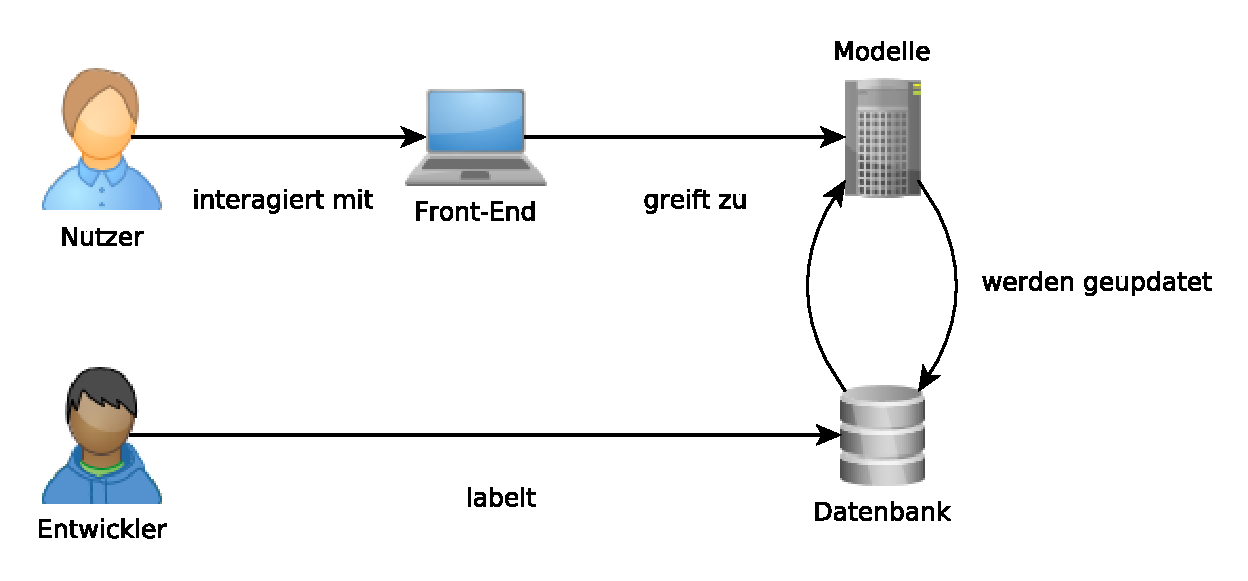
\includegraphics[width=\textwidth]{./Bilder/Sentiment/sentiment-architektur.pdf}
  \caption{Architektur aus Sicht des Sentiment-Pakets}
  \label{sentimentdetailarchitecture}
\end{figure}

Der Nutzer interagiert mit der Anwendung über das im Browser angezeigte Front-End. Seine Anfragen führen (via REST-Service) dazu, dass auf die Modelle zugegriffen wird, die auf der Festplatte liegen. Doch zeitgleich kann der Entwickler Tweets \texttt{labeln}, d.\,h., ihren Sentimentwert manuell bestimmen und so Trainingsdaten schaffen, um die Genauigkeit der Schätzungen zu verbessern. Deshalb müssen die Modelle aktuell gehalten werden, wenn neue Trainingsdaten vorliegen.

\texttt{Sentiment\-Label\-Tool} ist ein von der restlichen Anwendung unabhängiges Tool, das es ermöglicht, Tweets ohne direkten Zugriff auf die Datenbank und ohne Tools wie PHPMyAdmin zu labeln. Der Nutzer wählt die Sprache aus, in der Tweets gelabelt werden sollen. Dann wird ein Batch von 1000 Tweets geladen und der erste angezeigt. Der Nutzer gibt seine Bewertung in den Schritten -1, -0,5, 0, 0.5 oder 1 ein und bekommt anschließend den nächsten Tweet angezeigt. Tweets können auch übersprungen werden. Sobald zehn Tweets bearbeitet worden sind, wird der Batch vom Tool an die Datenbank gesendet und der nächste geholt. Der Grund für die unterschiedlichen Batch-Größen liegt darin, dass beim Laden 1000 zufällige Tweets ausgewählt werden. Diese Operation nimmt in MySQL einen sehr langen Zeitraum in Anspruch, dessen Dauer nicht von der Anzahl der abgefragten Tweets abhängt. Das Speichern von Sentimentwerten ist dagegen eine vergleichsweise schnelle Operation.

\label{sentimentupdater}

\texttt{Regression\-Sentiment\-Updater} läuft in einem eigenen Thread und kümmert sich um die Aktualisierung der Regressionsmodelle und die Sentiment-Aktualisierung aller Tweets in der Datenbank. Dazu überprüft er zunächst, ob neue Trainingsdaten zu einer beliebigen Sprache in der Datenbank vorhanden sind. Dies ist immer dann der Fall, wenn neue Tweets gelabelt worden sind. In diesem Fall wird eine Regression durchgeführt und das Modell gespeichert. Das Modell steht sofort als Java-Objekt dem \texttt{Regression\-Sentiment\-Classifier} zur Verfügung und wird für den Zugriff auch nach einem eventuellen Neustart des Daemons sowie für den REST-Service serialisiert und auf der Festplatte gespeichert. Anschließend wird das Sentiment aller Tweets in der Datenbank mit Hilfe des neuen Regressionsmodells berechnet und aktualisiert. Diese Überprüfung und die erneute Regression werden für alle Sprachen alle 24 Stunden durchgeführt. Das Programm ist somit selbst dafür zuständig, zu erkennen, ob es neue Modelle erstellen kann und es ist außer dem Labeln keine andere manuelle Intervention notwendig, um bessere Sentimentschätzungen zu erhalten.

\subsection{Diskussion}

Es lassen sich zwei Herausforderungen identifizieren, die sich bei der Umsetzung der Sentiment-Vorhersagen ergaben, nämlich die Überanpassung (\textit{overfitting}) und die Datenbankperformance. 

Voraussetzung für eine erfolgreiche Sentimentanalyse ist, dass die Sentimentwerte zu vielen Texten bereits bekannt sind. Die lineare Regression findet die optimalen Gewichte für die Vorhersage der Labels zu den Trainingsdaten. Dies bedeutet nicht notwendigerweise, dass neue Daten auch gut vorhergesagt werden. Der Begriff der Überanpassung an die Trainingsdaten beschreibt das Phänomen, dass Eigenheiten der Trainingsdaten, die nicht für andere Daten verallgemeinert werden können, vom Klassifikator zur Bewertung herangezogen werden. Überanpassung tritt auf, wenn die Zahl der Parameter bzw. Features zu hoch ist für die Anzahl der Datensätze.

Das heißt, dass die Überanpassung zu verringern ist, indem die Zahl der Datensätze erhöht oder die Zahl der Parameter gesenkt wird. Je mehr Trainingsdaten vorliegen, die zufällig aus dem Korpus ausgewählt sind, desto geringer wird der Einfluss einzelner Zufälle, aber Überanpassung kann nie ganz ausgeschlossen werden. Zum Beispiel könnte ein Begriff wie Irak auch über Jahre hinweg mit schlechten Nachrichten und erhitzten Debatten assoziiert sein. Mit diesen Daten trainiert, würde ein Klassifikator ihn (richtigerweise) zur Vorhersage negativer Emotion verwenden, und könnte vermutlich nicht verwendet werden, um Nachrichten über Irak aus einem anderen Themengebiet zu verwenden.

Die Überanpassung hat sich in diesem Projekt wie folgt geäußert: Zur Einschätzung des Sentimentwertes eines neuen Tweets können offensichtlich nur Features verwendet werden, die dem Modell bereits aus den Trainingsdaten bekannt sind. Obwohl mehr als 1000 manuell annotierte Tweets (deutsche und englische) als Trainingsdaten verwendet wurden, kam es regelmäßig vor, dass in den Testdaten Wörter vorkamen, die zweifellos zur emotionalen Aussage des Tweets beitrugen, aber nicht in den Trainingsdaten vorhanden gewesen waren und somit nicht zur Schätzung des Sentiments verwendet werden konnten. Das Feature wurde nicht erkannt, der entsprechende Parameterwert fehlt im Modell. Da bei einer linearen Regression mit n-Gramm-Features der Sentimentwert des Texts die Summe der Parameter der einzelnen n-Gramme ist, führt dieses Fehlen von Parameterwerten zu einer (absolut) zu niedrigen Schätzung.

Hinzu kommt, dass für den Algorithmus bei einem Mangel an Trainingsdaten nicht ersichtlich ist, welche Features für die Einschätzung des Sentimentwerts wichtig sind und welche nicht. Implizit werden häufige Features stärker gewichtet, denn wenn in einer Iteration des Gradientenabstiegsverfahrens der Parameterwert eines häufigen Features besser wird, hat dies einen höheren Einfluss auf den Fehler des Modells als bei einem seltenen Feature. Dieser Unterschied ist allerdings nur dann ausgeprägt, wenn ausreichend Trainingsdaten vorliegen. Wenn er nicht ausgeprägt ist, wie in unserem Fall, erhalten auch seltene Features, beispielsweise Fourgrams, vergleichsweise hohe Parameterwerte, und häufige Features vergleichsweise niedrige. Wird dieses Modell auf neue Daten angewandt, und werden dabei nur einige der vorliegenden Features erkannt, kommt es hierdurch wiederum verstärkt zu einer (absolut) zu niedrigen Schätzung. Es liegt ein Bias zugunsten absolut niedriger Sentimentwerte vor.

Zur Behebung des Problems wurden unterschiedliche Lösungsansätze versucht. Der vielversprechendste war, die Features auf all jene zu begrenzen, die mindestens in zwei Trainingsdatensätzen vorkamen. So nahmen wir zwar in Kauf, dass noch weniger Features wiedererkannt würden, erhofften uns aber auch, dass bei den tatsächlich wiedererkannten Features die Parameterwerte absolut höher sein würden. Dennoch ließ sich der Bias so nicht beseitigen.
Schließlich beschlossen wir, das Problem zu umgehen: Vorrangiges Ziel war die Einordnung der Tweets in negative, neutrale und positive. Diese Einordnung funktioniert trotz des Bias gut, wenn die Grenzen zwischen den Kategorien ebenfalls auf absolut niedrige Werte gesetzt werden.

Im Ergebnis empfehlen wir für den praktischen Einsatz die weitere Erhöhung der Zahl der Trainingstweets und möglicherweise die Verringerung der Anzahl Features mithilfe von Algorithmen zur \textit{feature selection}. Um den beschriebenen Bias zu verhindern, erscheinen nichtlineare Algorithmen vielversprechend, die besser mit dem Fehlen von Features umgehen können.

Neben der Überanpassung war die Datenbank-Performance eine Schwierigkeit. Gerade der \texttt{Regression\-Sentiment\-Updater} hat die komplexe Aufgabe, die Sentimentwerte aller Tweets in der Datenbank zu ändern, wenn neue Daten gelabelt worden sind. Im produktiven Einsatz kommt dies zwar kaum vor, während der Entwicklung dagegen umso häufiger. Bei mehreren Millionen Tweets nehmen die nötigen Datenbankoperationen eine große Menge Zeit und Ressourcen in Anspruch. Diese Aufgabe ist erfolgreich gelöst worden. Als hilfreich hat sich insbesondere das Profiling erwiesen, also das Aufzeichnen von Methodenlaufzeiten und verwendetem Speicher, um Bottlenecks zu identifizieren. Eine aktzeptable Laufzeit und ein geringer Speicherverbrauch wurden schließlich durch die Verwendung geeigneter \textit{batched statements} in Verbindung mit manuellen Commits sowie einem \textit{streaming result set}.